\documentclass[border=5pt]{standalone}
\usepackage{tikz}
\usetikzlibrary{arrows.meta, positioning, shapes.geometric}
\usepackage{xcolor}

\definecolor{Garnet}{HTML}{73000A}
\definecolor{NinetyBlack}{HTML}{363636}
\definecolor{SeventyBlack}{HTML}{5C5C5C}
\definecolor{TenBlack}{HTML}{ECECEC}

\begin{document}
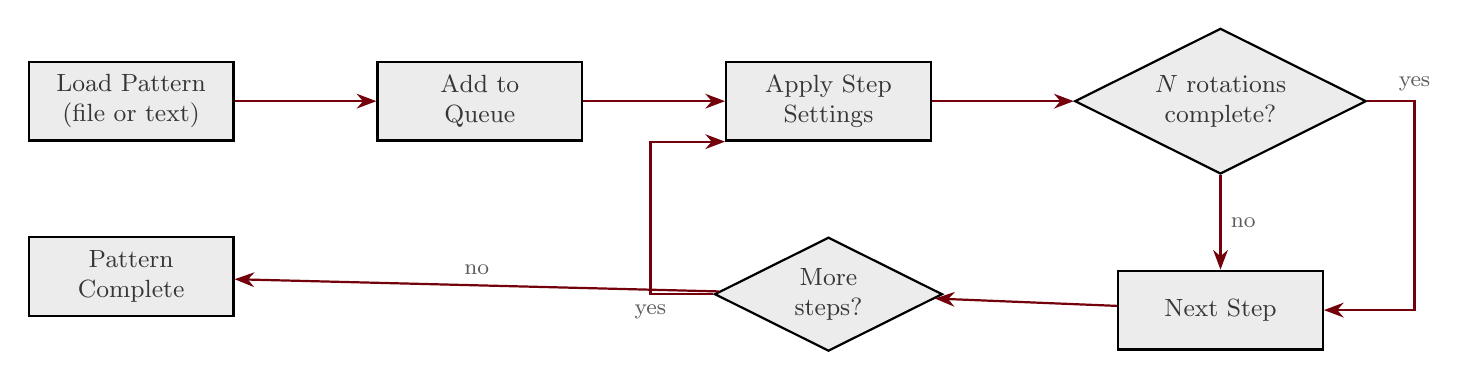
\begin{tikzpicture}[
    proc/.style={draw, thick, minimum width=2.6cm, minimum height=1cm, align=center, fill=TenBlack, text=NinetyBlack, font=\small},
    decision/.style={draw, thick, diamond, aspect=2, minimum width=2cm, align=center, fill=TenBlack, text=NinetyBlack, font=\small},
    arr/.style={-{Stealth[length=2.5mm]}, thick, Garnet},
    every node/.append style={rounded corners=0pt},
]
    \node[proc] (load) {Load Pattern\\(file or text)};
    \node[proc, right=1.8cm of load] (queue) {Add to\\Queue};
    \node[proc, right=1.8cm of queue] (apply) {Apply Step\\Settings};
    \node[decision, right=1.8cm of apply] (wait) {$N$ rotations\\complete?};
    \node[proc, below=1.2cm of wait] (next) {Next Step};
    \node[decision, below=1.2cm of apply] (more) {More\\steps?};
    \node[proc, below=1.2cm of load] (done) {Pattern\\Complete};

    \draw[arr] (load) -- (queue);
    \draw[arr] (queue) -- (apply);
    \draw[arr] (apply) -- (wait);
    \draw[arr] (wait.south) -- node[right, font=\footnotesize, text=SeventyBlack] {no} (next);
    \draw[arr] (wait.east) -- ++(0.6,0) node[above, font=\footnotesize, text=SeventyBlack] {yes} |- (next.east);
    \draw[arr] (next) -- (more);
    \draw[arr] (more) -- node[above, font=\footnotesize, text=SeventyBlack] {no} (done);
    \draw[arr] (more.west) -- ++(-0.8,0) node[below, font=\footnotesize, text=SeventyBlack] {yes} |- (apply.south west);
\end{tikzpicture}
\end{document}
